\documentclass{article}

%\begin{figure}[h]
%\begin{center}
%\caption{\label{1} titre}
%\includegraphics[scale=0.5]{{nom_photo}.png}
%\captionsetup{labelformat=empty}
%\caption{ sources : nom_source}
%\end{center}
%\end{figure}

% \begin{center}
% \begin{tabular}{|c|c|}
			% \hline
			% a & a \\
			
			% a & a  \\
			% \hline
			% a & a \\
			
			% a & a  \\
			% \hline
			% a & a \\
			
			% a & a  \\
			% \hline
% \end{tabular}
% \end{center}

%[ForwardSearch("%bm.pdf","%Wc",%l,0,0,1)]


\usepackage[utf8]{inputenc}
\usepackage[T1]{fontenc}
\usepackage[french]{babel}
\usepackage{amsmath}
\usepackage{amssymb}
\usepackage{graphicx}
\usepackage{caption}
\usepackage{subcaption}
\usepackage{fancyhdr}
\usepackage{gensymb}
\usepackage{array}
\usepackage{caption}
\usepackage[left=2cm,right=2cm,top=2cm,bottom=2cm]{geometry}
%\newgeometry{top=1in,bottom=1in,right=0.5in,left=1.5in}

\usepackage{listings}
\usepackage{color}

\definecolor{dkgreen}{rgb}{0,0.6,0}
\definecolor{gray}{rgb}{0.5,0.5,0.5}
\definecolor{mauve}{rgb}{0.58,0,0.82}

\lstset{frame=tb,
  language=Python,
  aboveskip=3mm,
  belowskip=3mm,
  showstringspaces=false,
  columns=flexible,
  basicstyle={\small\ttfamily},
  numbers=none,
  numberstyle=\tiny\color{gray},
  keywordstyle=\color{blue},
  commentstyle=\color{dkgreen},
  stringstyle=\color{mauve},
  breaklines=true,
  breakatwhitespace=true,
  tabsize=3
}

\renewcommand{\thesection}{\Roman{section}}
\renewcommand{\thesubsection}{\arabic{subsection}}


\newcommand{\deriv}[2]{\frac{\partial #1}{\partial #2}}
\DeclareMathOperator{\Tr}{Tr}
\title{Machine learning pour la classification de phases de sommeil}
\author{Alexandre Herbert et Baptiste Turpin}
\date{}
\begin{document}

\maketitle

\vspace{ 10\baselineskip}

\begin{figure}[h]
\begin{center}

\includegraphics[scale=0.55]{{images/CS}.jpeg}
%\hspace{50pt}

\includegraphics[scale=0.2]{{images/dreem_logo}.png}
\end{center}
\end{figure}

\newpage

\setcounter{tocdepth}{2}
\renewcommand{\contentsname}{Sommaire}
\tableofcontents

\newpage

\section{\hspace{0.3cm} Contexte}

Le sommeil tient une place majeure dans notre santé et notre bien-être. Il se décompose en une succession de phases répétées par cycle :
\\
\begin{itemize}
\item Phase 0 : endormissement (individu réveillé)
\item Phase 1 : sommeil léger
\item Phases 2 et 3 : sommeil profond
\item Phase 4 : sommeil paradoxal ou REM (Rapid Eye Movement)
\end{itemize}
\vspace{0.5cm}

Le travail de DREEM repose sur la mise en place de solutions permettant de diagnostiquer les problèmes de sommeil. Il s'agit d'identifier lors d'une session de sommeil l'enchainement des différentes phases pour comprendre l'origine du trouble. A cette fin, DREEM a lancé sur le marché un bandeau permettant de récupérer 3 catégories de signaux pendant le sommeil de l'individu :
\\
\begin{itemize}
\item L'activité éléctrique du cerveau (par 7 électroencéphalographie)
\item L'accélération (par 3 accéléromètrie)
\item L'absorption de la lumière infrarouge par l'hémoglobine, caractéristique de la teneur en oxygène du sang (par 1 oxymétrie colorimétrique)
\end{itemize}
\vspace{0.5cm}

L'objectif est de prédire la phase du sommeil à partir de ces 11 signaux relevés. À cette fin, DREEM travaille sur un modèle d'apprentissage supervisé pour la classification en 5 phases de sommeil. Des spécialistes du sommeil ont donc été sollicités pour étiqueter un ensemble d'échantillons, chaque échantillon étant constitué des 11 signaux capturés sur une période de 30 secondes.

\vspace{\baselineskip}

L'objectif du présent projet est :
\\
\begin{itemize}
\item De sélectionner un modèle de Machine Learning et des hyperparamètres efficaces pour le problème de classification proposé
\item D'identifier des features pertinents pour chacun des signaux permettant de discriminer les phases du sommeil
\item D'appliquer la technique d'apprentissage par validation croisée et un prétraitement des données adaptés au problème
\end{itemize}
\vspace{0.5cm}

Nous reviendrons dans ce qui suit sur les différents choix que nous avons opérés : modèle, prétraitement, extraction de features, entraînement. Nous présenterons ensuite de manière critique les résultats obtenus, avant d'envisager des perspectives d'amélioration.

\section{\hspace{0.3cm} Choix d'implémentation}
\subsection{Choix du modèle}

Dans un tout premier temps, nous avons utilisé un apprentissage non-supervisé de type k-means. Cette méthode, très peu performante, visait juste à évaluer la qualité des features extraits, pour savoir s'ils permettaient de discriminer efficacement les phases du sommeil. Aucune performance probante n'a pu être tirée de cette analyse.
\\

La lecture du rapport fourni nous a ensuite rapidement orienté vers les modèles évalués comme étant les plus performants pour ce problème : le Random Forest ou le simple Decision Tree.
\\

Nous nous sommes finalement tournés vers le Random Forest, afin d'obtenir une classification plus fine qu'un simple Decision Tree, et puisque nous ne cherchons pas ici à déterminer un sens "physique" pour les noeuds. Il en effet plus facile d'interpréter un simple arbre de décision d'après ses noeuds, tandis qu'un algorithme de Random Forest, générant une multitude d'arbres de décision aléatoires, sera plus difficilement interprétable. L'objectif était ici uniquement d'obtenir une classification efficace. Il aurait pu être intéressant (dans une optique de modélisation) de regarder au contraire des modèles interprétables.
\\

Nous avons cherché à optimiser les hyperparamètres suivants (attributs de la classe sklearn.ensemble.RandomForestClassifier) :
\\

\begin{itemize}
\item Le nombre d'arbres de la forêt (n\_estimators)
\item Le critère de qualité d'une division (criterion)
\item La profondeur maximale (max\_depth)
\item Le nombre minimal d'échantillons pour une division (min\_samples\_split)
\item Le nombre minimal d'échantillons par feuille (min\_samples\_leaf)
\item Le taux minimal de réduction du critère de qualité autorisant une division (min\_impurity\_decrease)
\end{itemize}
\vspace{0.5cm}



Finalement, les valeurs suivantes ont été choisies pour ces hyperparamètres :
\\

\begin{center}
 \begin{tabular}{|c|c|}
			 \hline
			 \textbf{Hyperparamètre} & \textbf{Valeur} \\
			 \hline
			 n\_estimators & 1000  \\
			 \hline
			 criterion & 'gini' \\
			 \hline
			 max\_depth & 16  \\
			 \hline
			 min\_samples\_split & 2 \\
			 \hline
			 min\_samples\_leaf & 1  \\
			 \hline
			 min\_impurity\_decrease & 0.0  \\
			 \hline
 \end{tabular}
\end{center}

\subsection{Description du modèle}

Le modèle du Random Forest consiste en un ensemble d'arbres de décision. Chaque arbre de décision est construit à partir d'un nombre restreint de features (relativement à l'ensemble des features) choisis aléatoirement. Sur chacun de ces arbres, on réalise alors une optimisation, dont le critère est l'impureté de Gini calculée aux feuilles de l'arbre. L'impureté à une feuille est nulle lorsque tous les éléments de cette feuille appartiennent à la même classe. La prédiction finale de l'algorithme Random Forest correspond ensuite au vote majoritaire de tous les arbres de décision générés.

\subsection{Sélection des méthodes de validation algorithmique}

L'optimisation des hyperparamètres (tant du modèle que des features extraits) est réalisée par validation croisée. Le découpage du dataset d'entrainement est réalisé avec la classe sklearn.model\_selection.StratifiedKFold. Le nombre de folds (n\_folds) a été fixé à 5. Le dataset est mélangé aléatoirement (shuffle = True).

Nous calculons à partir de cet apprentissage le F1-score ainsi que la matrice de confusion obtenus pour la validation.

\section{\hspace{0.3cm} Sélection de features}

Nous avons dans un premier temps affiché les signaux temporels du dataset d'entraînement afin d'établir des caractéristiques des différentes phases de sommeil et ainsi tenter de dégager des features pertinents.
\\

\begin{figure}[h]
\begin{center}
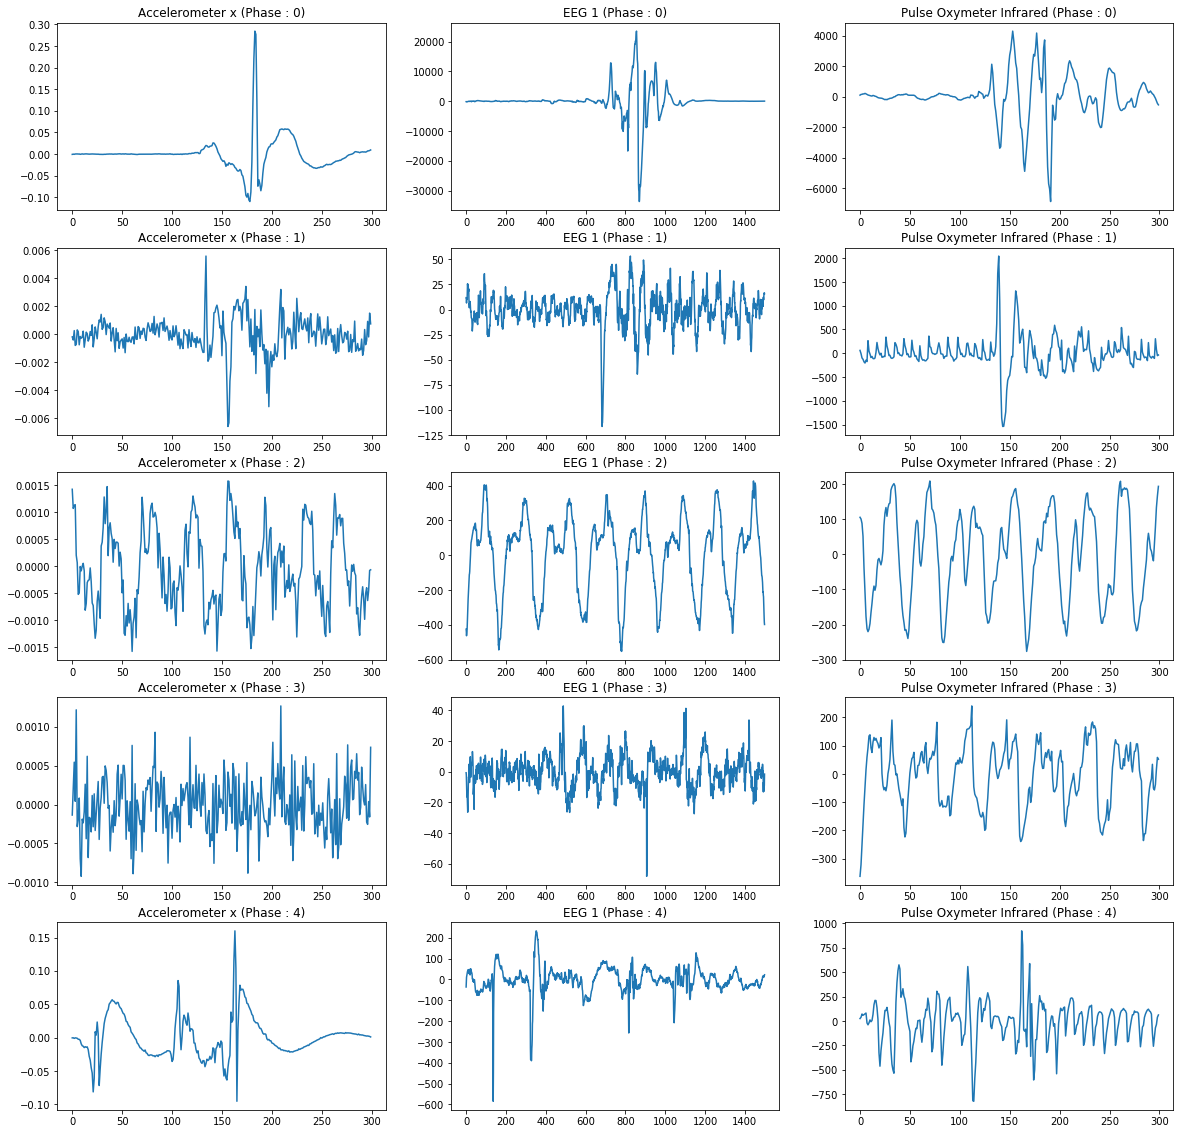
\includegraphics[scale=0.4]{{images/temp_signals}.png}
\caption{Signaux temporels pour différentes phases}
\end{center}
\end{figure}

\clearpage

Nous pouvons faire les premières observations suivantes :
\\

\begin{itemize}
\item Les signaux de la phase 0 sont d'amplitude très élevée, mais avec de faibles fluctuations, et sans motif répété.
\item L'accéléromètre de la phase 4 ne présente que peu de fluctuation, et aucun motif répété.
\end{itemize}
\vspace{0.5cm}

Plus généralement, on constate que :
\\

\begin{itemize}
\item Les signaux se composent de motifs répétés pour les phases 1, 2 et 3.
\item La forme des motifs, leur amplitude et leur fréquence d'apparition semble varier en fonction de la phase
\end{itemize}
\vspace{0.5cm}

Cela nous amène à considérer en supplément les caractéristiques fréquentielles des signaux. Nous avons calculé la valeur absolue de la transformée de Fourier des signaux temporels (figure 2).
\\


\begin{figure}[h]
\begin{center}
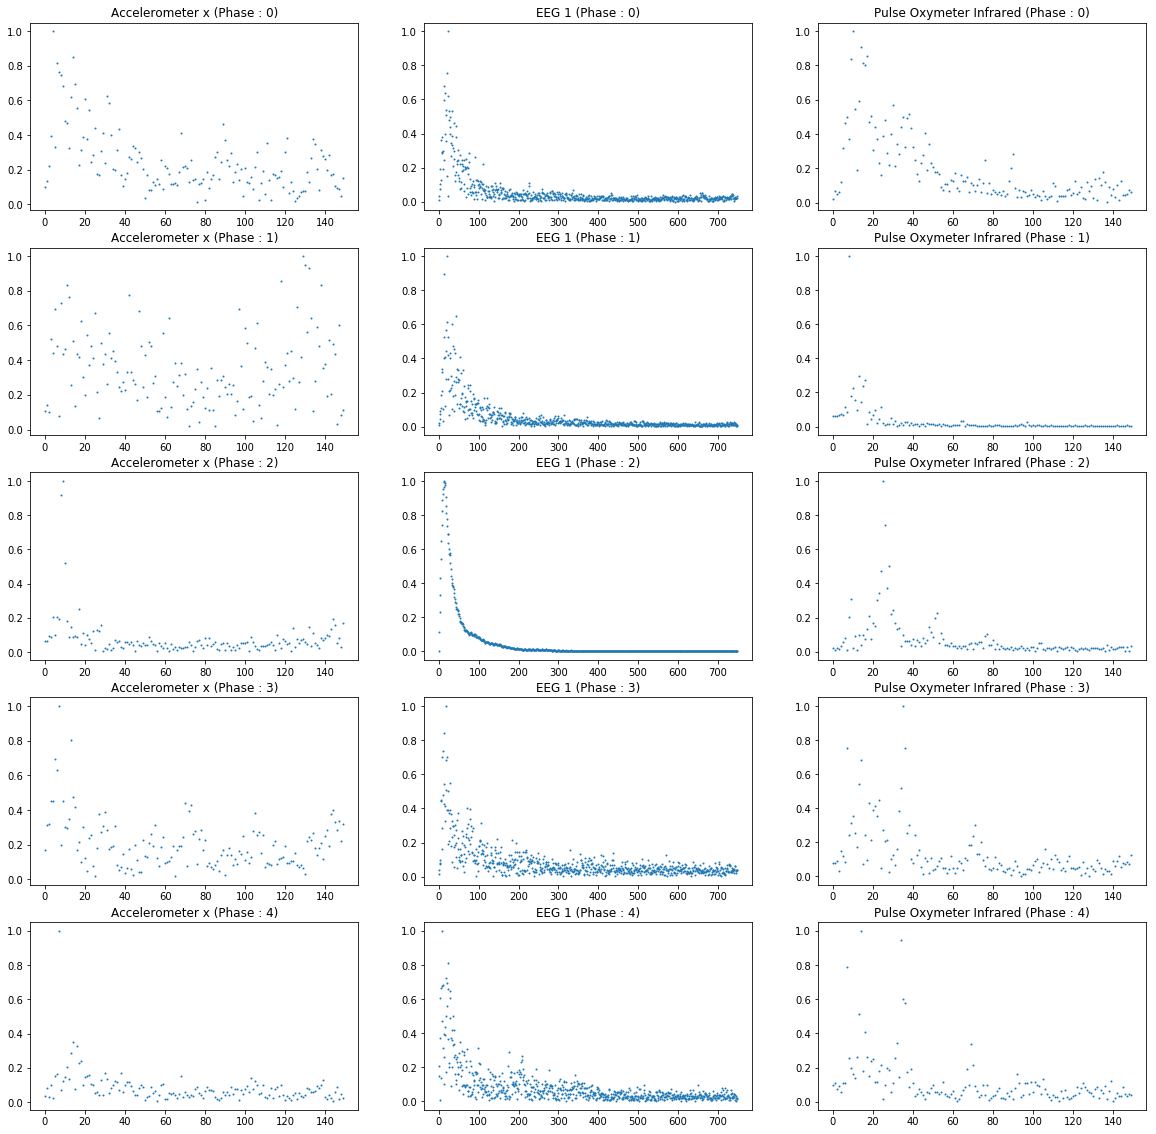
\includegraphics[scale=0.3]{{images/freq_signals}.png}
\caption{FFT des signaux pour différentes phases}
\end{center}
\end{figure}


On constate sur la comparaison des FFT que l'amplitude maximale observée varie beaucoup en fonction de la phase de sommeil. En outre, en ne considérant que la forme de la FFT et la distribution des points dans la fenêtre d'affichage, on tire les observations suivantes :
\\

\begin{itemize}
\item EEGs : la FFT est plus ou moins bien dessinée en fonction de la phase : pour une plage de fréquences réduite donnée, il semblerait que la variance en amplitudes des différents points soit plus ou moins forte selon la phase de sommeil. Dans le cas ci-dessus, la phase 2 présente un écart-type faible sur toute plage de fréquences réduite, tandis que les phases 3 et 4 présentent un nuage de points plus étendu.
\item Accéléromètres : des points isolés en haut à droite de la fenêtre d'affichage peuvent être observés sur les phases 0, 1 et 3.
\item Oxymétrie colorimétrique : on distingue plusieurs pics, qui sont plus ou moins espacés et d'amplitudes plus ou moins équilibrées en fonction des phases.
\end{itemize}
\vspace{0.5cm}

De toutes ces observations, nous avons décidé d'extraire les features suivants. Dans la description, "signal" est la liste des ordonnées du signal : ordonnées temporelles (resp fréquentielles), suivant que la méthode est appliquée au signal temporel (resp à la transformée de Fourier) ). Par ailleurs, pour réduire l'impact des outliers, on considèrera pour certaines fonctions la moyenne mobile du signal (sur une largeur donnée $W$), notée $moving\_mean(signal)$ :
\\

\textbf{distanceMinMax} \\
Cette fonction retourne la somme des distances géométriques entre les points d'ordonnées minimum et maximum du signal, sur un découpage d'intervalles régulier.\\\\

\textbf{maxAmp} \\
Cette fonction retourne le maximum de la liste donnée en entrée.\\
maxAmp = $max(signal)$ \\\\

\textbf{freqMinLimitAmp} \\
Soit une amplitude A donnée. \\
Pour cette amplitude A, la fonction retourne l'abscisse $i_{min}$ (ie l'indice) minimal vérifiant $\forall i > i_{min}, signal(i)< A$\\\\

\textbf{nbPikes} \\
Soit une amplitude A et une largeur d'intervalle W données.\\

On définit un pic au seuil A par l'ensemble des points voisins au dessus de ce seuil. \\
nbPikes est le nombre de pics distincts de $moving\_mean(signal,W)$. \\

\textbf{indexMaxAmp} \\
Soit une largeur d'intervalle W. \\
Cette fonction retourne l'abscisse i de la valeur maximale de $moving\_mean(signal,W)$. \\


\textbf{meanDiffNeighb} \\
Cette fonction retourne la moyenne des écarts (en valeur absolue) entre points voisins du signal. \\


\textbf{stdDeviationNb} \\
Cette fonction retourne la moyenne des écarts-type calculés séparément sur un découpage d'intervalles réguliers. \\

\textbf{upperRight} \\
Soit une amplitude A et une abscisse i. Cette fonction retourne le nombre de points observés dans le cadre supérieur droit délimité par l'abscisse i et l'amplitude A.\\

upperRight = $\sum\limits_{a>i}(\mathbf{1}(signal(a)>A))$.\\

\textbf{mean} \\
Cette fonction retourne la moyenne du signal.\\
mean = mean(signal)\\

\textbf{meanOfAbs} \\
Cette fonction retourne la moyenne de la valeur absolue du signal.\\
meanOfAbs = mean(abs(signal))\\

\textbf{maxOfAbs} \\
Cette fonction retourne le maximum de la valeur absolue du signal.\\
maxOfAbs = max(abs(signal))\\

\textbf{minOfAbs} \\
Cette fonction retourne le minimum de la valeur absolue du signal.\\
minOfAbs = min(abs(signal))

\section{\hspace{0.3cm} Pré-traitement des données}

Nous avons dans un premier temps pu constater que le dataset d'entrainement est déséquilibré :
\\


\begin{figure}[h]
\begin{center}
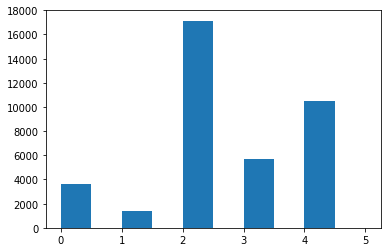
\includegraphics[scale=0.5]{{images/hist}.png}
\caption{Distribution du dataset d'entrainement entre les classes}
\end{center}
\end{figure}


Pour cette raison, nous avons appliqué deux méthodes :\\

\begin{itemize}
\item Réaliser la validation croisée sur un dataset équilibré entre les classes : tous les échantillons de la classe 1 (la moins représentée avec 1353 échantillons) sont conservés ; les échantillons des autres classes sont tirés aléatoirement. On passe ainsi d'un dataset de 38289 échantillons à un nouveau dataset équilibré de 6765 échantillons. 
\item Réaliser la validation croisée sur l'ensemble du dataset, et appliquer des poids aux classes pour pénaliser les mauvais classements associés aux classes les moins représentées.
\end{itemize}
\vspace{0.5cm}

Par ailleurs, la valeur absolue de la transformée de Fourier d'un signal est symétrique. Nous pouvons donc nous contenter de la première moitié de cette transformée de Fourier. \\

Enfin, pour certains features, on désire extraire de l'information dans la forme du signal ou de la transformée de Fourier. Dans ce cas précis, les amplitudes sont normalisées dans la fourchette [-1,1].\\

\section{\hspace{0.3cm} Optimisation des hyperparamètres des features}

Certains features listés plus tôt présentent des hyperparamètres : amplitude, largeur d'intervalle, abscisse. Nous avons décidé d'optimiser les valeurs de ces hyperparamètres séparément. Nous avons donc réalisé des apprentissages par validation croisée pour toutes les matrices de design élémentaires. Chaque matrice de design élémentaire est constituée d'un seul feature, appliqué à une seule catégorie de signal (EEG, accéléromètre ou oxymétrie colorimétrique), sur le signal temporel ou sur la transformée de Fourier.\\
On récupère ensuite la valeur des hyperparamètres maximisant le F1-score obtenu par validation croisée pour cette matrice de design.\\

Le but de cette optimisation est double :\\
\begin{itemize}
\item Identifier les features qui apportent les meilleurs résultats (ie dont le score-F1 atteint est le plus élevé)
\item Trouver, pour les features pertinents, les valeurs des hyperparamètres optimaux
\end{itemize}
\vspace{0.5cm}

Voici ci-dessous un extrait de l'analyse opérée :\\

\begin{figure}[h]
\begin{center}
\includegraphics[scale=0.3]{"images/optim".jpeg}
\caption{Extrait du tableau d'optimisation : scores F1 et valeurs des hyperparamètres optimaux associés}
\end{center}
\end{figure}



\section{\hspace{0.3cm} Résultats}

L'éxecution du script Python après écriture des différentes étapes listées ci-dessus nous a permis d'obtenir, sur le dataset de test utilisé sur Kaggle, un F1-score de 0.59752. Pour obtenir ce score, nous avons toutefois décidé d'utiliser finalement le dataset d'entraînement en entier, non ré-équilibré comme nous prévoyions de le faire. En effet, l'inconvénient de cette idée est qu'elle réduit fortement la taille du dataset d'entraînement (passant de 38289 à 6765 échantillons au total). Ainsi, le classifier, moins bien entraîné, fournit des résultats médiocres, inférieurs aux résultats de référence donnés sur Kaggle (``Random Forest on dummy features''). Par ailleurs, ce résultat fut obtenu en gardant tous les features (220 au total), car c'est cette configuration qui donna les meilleurs résultats. Nous avons cependant tenté de ne garder que ceux qui semblaient les plus pertinents (au vu du F1-score obtenu sur ces features seuls), mais tout retrait de features entrainait une diminution du F1-score obtenu. Il est à noter que l'optimisation réalisée au préalable nous a tout de même permis de déterminer les hyperparamètres optimaux des fonctions d'extraction de features.


\section{\hspace{0.3cm} Critiques et perspectives}

Comme expliqué précédemment, nous avons optimisé les hyperparamètres des features en validation croisée. En travaillant ainsi, nous savions qu'il y avait un risque d'overfitter les set de validation. Ce phénomène s'est révélé être bien plus important que nous ne le craignions, et le F1-score obtenu sur le dataset de test était nettement plus faible que celui obtenu en validation croisée.

\vspace{\baselineskip}

Nous aurions pu étudier d'autres modèles que le Random Forest. D'après le rapport fourni, les méthodes SVM et réseaux de neurones avaient en effet des performances proches de la méthode Random Forest.

\vspace{\baselineskip}

Par ailleurs, nous estimons que certains des features choisis pouvaient être corrélés, ce qui diminue leur valeur dans l'apprentissage et fait tendre vers l'overfitting. Pour pallier à ce problème, nous aurions pu calculer les matrices de corrélation afin d'identifier les features corrélés et ne sélectionner que les plus pertinents. On peut noter cependant que le fait d'utiliser un algorithme de Random Forest permet de limiter l'overfitting sur les features.

\vspace{\baselineskip}

Du point de vue de la société DREEM, il pourrait également être envisageable dans la mise au point de l'algorithme de classification de prendre en compte l'historique des phases de sommeil : la connaissance de la phase de sommeil correspondant au signal précédent peut grandement aider à la détermination du signal actuel.

\vspace{\baselineskip}

Enfin, les données nous ayant été fournies étant des données brutes, il serait possible de les traiter de manière plus poussée que ce que l'on a fait. Sont envisageables notamment de ce point de vue : suppression des outliers, filtrage à l'aide d'un filtre passe-bande, filtrage pour la réduction du bruit.


\newpage
\section{\hspace{0.3cm} Annexe : code Python}

\subsection{Script principal}
\begin{lstlisting}
## Imports
from feature_extraction import *
from feature_extraction_v2 import *
from ml_methods import myRandomForestClassifier
from cross_validation_learning import *

import numpy as np
import matplotlib.pyplot as plt
import h5py

## Parameters
create_new_design_matrix = True
create_new_prediction = True

name = 'prediction'

mlMethod = myRandomForestClassifier

labels_path = 'balanced_data/X_train_balanced_labels.txt'


n_estimators=[1000]  #[10, 100, 1000]
criterion=['gini']  #['gini', 'entropy']
max_depth=[16]
min_samples_split=[2]  #[2, 1000,500]
min_samples_leaf=[1]   #[1, 1000, 500] 
min_impurity_decrease=[0.0]

n_folds=5

list_params_tree = [n_estimators, criterion, max_depth, min_samples_split, min_samples_leaf, min_impurity_decrease]

list_params_tree_everything = [*n_estimators, *criterion, *max_depth, *min_samples_split, *min_samples_leaf, *min_impurity_decrease]

## Methods to be used
list_methods_time = [ distanceMinMaxOne , maxAmpOne , freqMinLimitAmpOne , nbPikesOne , indexMaxAmpOne , meanDiffNeighbOne , stdDeviationNbOne , meanOne , meanOfAbsOne , maxOfAbsOne , minOfAbsOne ]

list_methods_freq = [ distanceMinMaxOne , maxAmpOne , freqMinLimitAmpOne , nbPikesOne , indexMaxAmpOne , meanDiffNeighbOne , stdDeviationNbOne , meanOne , minOfAbsOne ]

## Temporal matrices

mat_bool_extract_signal_temp = np.array([  [0]*3 + [1]*7 + [0]  ,
                                           [0]*3 + [0]*7 + [0]  ,
                                           [0]*3 + [0]*7 + [1]  ,
                                           [0]*3 + [1]*7 + [1]  ,
                                           [0]*3 + [0]*7 + [0]  ,
                                           [1]*3 + [1]*7 + [0]  ,
                                           [1]*3 + [1]*7 + [0]  ,
                                           [0]*3 + [0]*7 + [0]  ,
                                           [1]*3 + [1]*7 + [0]  ,
                                           [0]*3 + [0]*7 + [0]  ,
                                           [0]*3 + [0]*7 + [0]    ])

 

                                           
mat_param_extract_signal_temp = np.array([  [[2]]*3 + [[5]]*7 + [[42]]  ,
                                           [[]]*3 + [[]]*7 + [[]]  ,
                                           [[0.44]]*3 + [[0.18]]*7 + [[0.57]]  ,
                                           [[18,0.2105]]*3 + [[2, 0.0526]]*7 + [[16,0.3367]]  ,
                                           [[11]]*3 + [[31]]*7 + [[18]]  ,
                                           [[1]]*3 + [[1]]*7 + [[1]]  ,
                                           [[42]]*3 + [[6]]*7 + [[44]]  ,
                                           [[]]*3 + [[]]*7 + [[]]  ,
                                           [[]]*3 + [[]]*7 + [[]]  ,
                                           [[]]*3 + [[]]*7 + [[]]  ,
                                           [[]]*3 + [[]]*7 + [[]]    ])

n,m = mat_param_extract_signal_temp.shape
for i in range(n):
    for j in range(m):
        if not mat_bool_extract_signal_temp[i,j]:
            mat_param_extract_signal_temp[i,j] = None

## Frequential matrices

mat_bool_extract_signal_freq = np.array([  [0]*3 + [1]*7 + [0]  ,
                                           [1]*3 + [1]*7 + [0]  ,
                                           [0]*3 + [0]*7 + [1]  ,
                                           [0]*3 + [0]*7 + [0]  ,
                                           [0]*3 + [0]*7 + [1]  ,
                                           [1]*3 + [1]*7 + [1]  ,
                                           [1]*3 + [1]*7 + [0]  ,
                                           [1]*3 + [1]*7 + [0]  ,
                                           [0]*3 + [0]*7 + [0]    ])

                                    
mat_param_extract_signal_freq = np.array([  [[2]]*3 + [[19]]*7 + [[16]]  ,
                                           [[]]*3 + [[]]*7 + [[]]  ,
                                           [[0.87]]*3 + [[0.09]]*7 + [[0.97]]  ,
                                           [[1,0.2105]]*3 + [[1, 0.0526]]*7 + [[7,0.1053]]  ,
                                           [[1]]*3 + [[17]]*7 + [[5]]  ,
                                           [[1]]*3 + [[1]]*7 + [[1]]  ,
                                           [[50]]*3 + [[22]]*7 + [[20]]  ,
                                           [[]]*3 + [[]]*7 + [[]]  ,
                                           [[]]*3 + [[]]*7 + [[]]    ])

nf,mf = mat_param_extract_signal_freq.shape
for i in range(nf):
    for j in range(mf):
        if not mat_bool_extract_signal_freq[i,j]:
            mat_param_extract_signal_freq[i,j] = None

## Importing data
X_train_balanced = h5py.File('balanced_data/X_train_balanced.h5' , 'r' )

X_train_fft_balanced = h5py.File('balanced_data/X_train_fft_balanced.h5' , 'r' )


X_test = h5py.File('data/X_test.h5')

X_test_fft = h5py.File('data/X_test_fft.h5')

## Creating the design matrices
if create_new_design_matrix:
    matrix_temp = extractMultiFeatureAllAdapt(X_train_balanced , list_methods_time , mat_bool_extract_signal_temp , mat_param_extract_signal_temp , save = True , name_save = "big_matrix_" + name + "_temp")
    
    matrix_freq = extractMultiFeatureAllAdapt(X_train_fft_balanced , list_methods_freq , mat_bool_extract_signal_freq , mat_param_extract_signal_freq , save = True , name_save = "big_matrix_" + name + "_freq")
    
    matrix = concatenateDesignMatrices( matrix_temp , matrix_freq , name_save = "big_matrix_" + name )

## Importing from previous calculations
else:
    matrix = objectFromFile("design_matrix/big_matrix_" + name + ".txt")

## Creating design matrix for prediction
if create_new_prediction:
    prediction_matrix_temp = extractMultiFeatureAllAdapt(X_test , list_methods_time , mat_bool_extract_signal_temp , mat_param_extract_signal_temp , save = True , name_save = "big_prediction_matrix_" + name + "_temp")
    
    prediction_matrix_freq = extractMultiFeatureAllAdapt(X_test_fft , list_methods_freq , mat_bool_extract_signal_freq , mat_param_extract_signal_freq , save = True , name_save = "big_prediction_matrix_" + name + "_freq")
    
    
    prediction_matrix = concatenateDesignMatrices( prediction_matrix_temp , prediction_matrix_freq , name_save = "big_prediction_matrix_" + name )

else:
    prediction_matrix = objectFromFile("design_matrix/big_prediction_matrix_" + name + ".txt" )


## Learning


mat_theta , mat_ypred , mat_yprob  = learn( matrix , mlMethod , list_params_tree , n_folds , labels_path = labels_path)

clf , scaler = learnEverything( matrix , mlMethod , list_params_tree_everything , labels_path = labels_path )

## Visualizing

visualizeResults( mat_theta , mat_ypred , mat_yprob , 0 , "" , [0,0,0,0,0] , labels_path = labels_path )

## Predicting

predict( prediction_matrix , clf , scaler = scaler , save = True , name_save =  name)
\end{lstlisting}

\subsection{Extraction de features}
\begin{lstlisting}
import numpy as np
import pickle
import sys

## Auxiliary functions
def meanOfInterval(signal, freq_min, freq_max):
    return np.average(signal[freq_min:freq_max])
    
def buildIntervals(list_length, interval_width):
    return list([i, i+interval_width] for i in range(0,list_length,interval_width))

def mobilMean(signal , interval_width):  #use an odd number as interval_width, otherwise the width will be interval_width + 1.
    cumsum = np.cumsum(np.insert(signal, 0, 0)) 
    return (cumsum[interval_width:] - cumsum[:-interval_width]) / float(interval_width)


## methodOne(s) : feature-extraction methods

def distanceMinMaxOne( list_freq = None , param = None , rep_dim_feature_per_signal = False):  # param = [ interval_width ]
    # Returns the sum of distances betwwen the minimum and the maximum on a given set of intervals. Intended to be used with the temporal signal
    if rep_dim_feature_per_signal:
        return 1
    interval_width, = param
    i_max = len(list_freq)//interval_width
    return [ sum( np.linalg.norm( np.array([np.argmax(list_freq[i*interval_width:(i+1)*interval_width]) , max(list_freq[i*interval_width:(i+1)*interval_width])]) - np.array( [np.argmin(list_freq[i*interval_width:(i+1)*interval_width]) , min(list_freq[i*interval_width:(i+1)*interval_width])]) )  for i in range(i_max) ) ]  

def maxAmpOne(list_freq = None, param = None , rep_dim_feature_per_signal = False):  # param useless
    # Returns the maximum amplitude of a list of frequencies
    if rep_dim_feature_per_signal:
        return 1
    return [max(list_freq)]


def freqMinLimitAmpOne(list_freq = None, param = None , rep_dim_feature_per_signal = False):  # param = [amp_lim]
    # Returns the (minimum) frequency above which all frequencies have amplitude < amp_lim = param[0]
    if rep_dim_feature_per_signal:
        return 1
    
    amp_lim, = param
    normalized_list_freq = 1/max(abs(list_freq))*list_freq
    for i in range(len(normalized_list_freq)-1,-1,-1):
        if normalized_list_freq[i] > amp_lim:
            return [i+1]
    return [0]



def nbPikesOne(list_freq = None, param = None , rep_dim_feature_per_signal = False ):   #param = [interval_width, amp_lim]
    # Returns the number of frequency pikes for a given (amp_lim) amplitude, averaging with a mobile mean
    if rep_dim_feature_per_signal:
        return 1
    interval_width, amp_lim = param
    mobil_mean_list_freq = mobilMean(list_freq , interval_width)
    mobil_mean_list_freq = 1/max(abs(mobil_mean_list_freq))*mobil_mean_list_freq
    nb_pikes = 0
    
    
    is_interval_in_a_pike = 4   #code : 1 = [T,T] , 2 = [T,F] , 3 = [F,T] , 4 = [F,F]
    for i in range(len(mobil_mean_list_freq)):
        if mobil_mean_list_freq[i] > amp_lim:
            is_interval_in_a_pike = 1 if is_interval_in_a_pike in [1,2] else 2
        else:
            is_interval_in_a_pike = 3 if is_interval_in_a_pike in [1,2] else 4
        if is_interval_in_a_pike==2:
            nb_pikes+=1
    return [nb_pikes]


def nbPikesFastOne(list_freq = None, param = None , rep_dim_feature_per_signal = False ):   #param = [interval_width, amp_lim]
    # Returns the number of frequency pikes for a given (amp_lim) amplitude, averaging over an interval
    if rep_dim_feature_per_signal:
        return 1
    interval_width, amp_lim = param
    intervals = buildIntervals(len(list_freq), interval_width)
    normalized_list_freq = 1/max(abs(list_freq))*list_freq
    nb_pikes = 0
    is_interval_in_a_pike = [False , False]
    # for minim, maxim in intervals:
    #     mean_value = meanOfInterval(list_freq, minim, maxim)
    #     if mean_value > amp_lim:
    #         is_interval_in_a_pike = [True , is_interval_in_a_pike[0] ]
    #     else:
    #         is_interval_in_a_pike = [False , is_interval_in_a_pike[0] ]
    #     if not(is_interval_in_a_pike[1]) and is_interval_in_a_pike[0]:
    #         nb_pikes+=1
    
    is_interval_in_a_pike = 4   #code : 1 = [T,T] , 2 = [T,F] , 3 = [F,T] , 4 = [F,F]
    for minim, maxim in intervals:
        mean_value = meanOfInterval(normalized_list_freq, minim, maxim)
        if mean_value > amp_lim:
            is_interval_in_a_pike = 1 if is_interval_in_a_pike in [1,2] else 2
        else:
            is_interval_in_a_pike = 3 if is_interval_in_a_pike in [1,2] else 4
        if is_interval_in_a_pike==2:
            nb_pikes+=1
    return [nb_pikes]


def indexMaxAmpOne(list_freq = None , param = None , rep_dim_feature_per_signal = False):  # param = [ interval_width ]
    # Give the index of maximum amplitude, for the data averaged with a mobile mean of size interval_width
    if rep_dim_feature_per_signal:
        return 1
    interval_width, = param
    mobil_mean_list_freq = mobilMean(list_freq , interval_width)
    return [np.argmax(mobil_mean_list_freq)]

def indexMaxAmpFastOne(list_freq = None , param = None , rep_dim_feature_per_signal = False):  # param = [ interval_width ]
    # Give the index of maximum amplitude, for the data averaged over fixed intervals. Probably way faster than indexMaxAmpOne, though less accurate.
    if rep_dim_feature_per_signal:
        return 1
    interval_width, = param
    i_max = len(list_freq)//interval_width
    #side_interval = interval_width//2
    list_mean = list( np.average( list_freq[i*interval_width:(i+1)*interval_width]) for i in range(i_max) )
    return [ np.argmax(list_mean)*interval_width + interval_width//2 ]


def meanDiffNeighbOne(list_freq = None , param = None , rep_dim_feature_per_signal = False):  #param = [interval_width]  (for moving mean
    # Returns the average of absolute difference of amplitude between all neighbours frequencies
    if rep_dim_feature_per_signal:
        return 1
    
    interval_width, = param
    moving_mean_list = mobilMean(list_freq , interval_width) if interval_width>1 else list_freq.copy()
    return [np.average(list(abs(moving_mean_list[i+1]-moving_mean_list[i]) for i in range(len(moving_mean_list)-1)))]


    
def stdDeviationNbOne(list_freq = None , param = None , rep_dim_feature_per_signal = False ):  #param = [ n_nb ]
    # Returns the average of standard deviations computed on a given number of points (separation of x-axis in intervals of the same length)
    if rep_dim_feature_per_signal:
        return 1
    n_nb, = param
    c_max = len(list_freq)//n_nb
    return [np.average(list(np.std(list_freq[c*n_nb:(c+1)*n_nb]) for c in range(c_max)))]

    
def upperRightOne(list_freq = None , param = None , rep_dim_feature_per_signal = False):   # param = [th_amp , th_freq]
    # Returns the number of points in the upper right corner defined by the parameters
    if rep_dim_feature_per_signal:
        return 1
        
    normalized_list_freq = 1/max(abs(list_freq))*list_freq
    th_amp , th_freq = param
    index_th_freq = int(th_freq*(len(list_freq)-1))
    
    
    return([len(([amp for amp in normalized_list_freq[index_th_freq:] if amp > th_amp]))])
        

def meanOne(list_time = None , param = None , rep_dim_feature_per_signal = False): # param is useless
    # Returns the mean of the signal
    if rep_dim_feature_per_signal:
        return 1
    return [np.mean(list_time)]

def meanOfAbsOne(list_time = None , param = None , rep_dim_feature_per_signal = False):  # param is useless
    # Returns the mean of the signal's absolute value
    if rep_dim_feature_per_signal:
        return 1

    return [np.mean(np.abs(list_time))]
    
def maxOfAbsOne(list_time = None , param = None , rep_dim_feature_per_signal = False):  # param is useless
    # Returns the mean of the signal's absolute value
    if rep_dim_feature_per_signal:
        return 1

    return [np.max(np.abs(list_time))]

def minOfAbsOne(list_time = None , param = None , rep_dim_feature_per_signal = False):  # param is useless
    # Returns the mean of the signal's absolute value
    if rep_dim_feature_per_signal:
        return 1

    return [np.min(np.abs(list_time))]


## Global feature-extraction methods
    
def extractFeatureAll(h5file_freq , methodOne , param , list_bool_extract_signal):
    # Method giving the design matrix of h5file, given a certain method
    # list_bool_extract_signal[i] contains 1 iff the ith signal (data field) must have its feature extracted for this methodOne. Must be of length : len(key_list)
    key_list = list(h5file_freq.keys())
    key_list_extract = list( key_list[i] for i in range(len(key_list)) if list_bool_extract_signal[i] )
    nb_samples = len(h5file_freq[key_list[0]])
    dim_feature_per_signal = methodOne(rep_dim_feature_per_signal = True)
    rep = np.zeros((nb_samples , len(key_list_extract)*dim_feature_per_signal))
    
    for k_id in range(len(key_list_extract)):
        k=key_list_extract[k_id]
        rep[: ,k_id*dim_feature_per_signal:(k_id+1)*dim_feature_per_signal ] =  np.array( list(methodOne(h5file_freq[k][i] , param) for i in range(nb_samples)  ))
    return rep

def extractMultiFeatureAll(h5file_freq , list_methodOne , list_param , mat_bool_extract_signal , save = False , name_save = None):
    # Returns the concatenation of design matrices for a list of methods
    # mat_bool_extract_signal[i] (ith row) contains list_bool_extract_signal for extractFeatureAll function. IE : mat_bool_extract_signal[i,j] is 1 iff for ith methodOne, jth signal must have its feature extracted. 
    # mat_bool_extract_signal must be of size : (nb of methodOnes , len(key_list)  )
    key_list = list(h5file_freq.keys())
    nb_samples = len(h5file_freq[list(h5file_freq.keys())[0]])
    #sum_dim_feature_per_signal = sum( methodOne(rep_dim_feature_per_signal = True) for methodOne in list_methodOne )
    
    list_key_list_extract = list( list( key_list[j] for j in range(len(key_list)) if mat_bool_extract_signal[i,j] ) for i in range(len(list_methodOne)) )
    
    sum_weighted_dim_feature_per_signal = sum( list_methodOne[i](rep_dim_feature_per_signal = True)*len(list_key_list_extract[i]) for i in range(len(list_methodOne)) )
    
    rep = np.zeros((nb_samples , sum_weighted_dim_feature_per_signal ))
    
    c = 0
    i = 0
    
    # setup toolbar
    print("Progress...")
    sys.stdout.write("|"+("_" * len(list_methodOne)) + "_|\n")
    sys.stdout.flush()
    sys.stdout.write("|>")
    sys.stdout.flush()
    
    for methodOne in list_methodOne :
        
        # update the bar
        sys.stdout.write("\b")
        sys.stdout.write("=>")
        sys.stdout.flush()
        
        temp = len(list_key_list_extract[i])*methodOne(rep_dim_feature_per_signal = True)
        rep[:,c:c+temp] = extractFeatureAll(h5file_freq , methodOne , list_param[i] , mat_bool_extract_signal[i] )
        i+=1
        c+=temp
    
    # close the bar
    sys.stdout.write("\b")
    sys.stdout.write("=|\n")
    
    if save:
        temp_var_file = open("design_matrix/" +name_save + '.txt','wb')
        pickle.dump(rep , temp_var_file)
        temp_var_file.close()
        
        #Use next 3 lines to read
        # temp_var_file = open(name_save + '.txt','rb')
        # rep = pickle.load(temp_var_file)
        # temp_var_file.close()
        
        #np.savetxt( name_save + '.txt' , rep , delimiter=',', fmt="%s")
    
    return rep

## File handling

def objectFromFile( file_path ):
    temp_var_file = open(file_path ,'rb')
    rep = pickle.load(temp_var_file)
    temp_var_file.close()
    return rep

def concatenateDesignMatricesFromPath( file_path1 , file_path2 , name_save = None ):
    rep = np.concatenate( (objectFromFile(file_path1), objectFromFile(file_path2)) , axis = 1)
    if not name_save is None:
        temp_var_file = open("design_matrix/" + name_save + '.txt','wb')
        pickle.dump(rep , temp_var_file)
        temp_var_file.close()
    return rep

def concatenateDesignMatrices( mat1 , mat2 , name_save = None ):
    rep = np.concatenate( (mat1 , mat2) , axis = 1)
    if not name_save is None:
        temp_var_file = open("design_matrix/" + name_save + '.txt','wb')
        pickle.dump(rep , temp_var_file)
        temp_var_file.close()
    return rep

def labelsCsv2Txt( file_path , name_save ):
    labels = np.loadtxt(file_path,  delimiter=',', skiprows=1, usecols=range(1, 2)).astype('int')
    temp_var_file = open('data/' + name_save + '.txt','wb')
    pickle.dump(labels , temp_var_file)
    temp_var_file.close()

\end{lstlisting}

\subsection{Méthode de Cross-validation}

\begin{lstlisting}

from feature_extraction import objectFromFile

import numpy as np
import sklearn
#from sklearn import neighbors
#from sklearn import cross_validation
from sklearn import model_selection
from sklearn import cluster
from sklearn import svm
from functools import reduce
import operator
import matplotlib.pyplot as plt
import csv
import sys

def cross_validate(design_matrix, labels, classifier, n_folds):
    """ Perform a cross-validation and returns the predictions.
    
    Parameters:
    -----------
    design_matrix: (n_samples, n_features) np.array
        Design matrix for the experiment.
    labels: (n_samples, ) np.array
        Vector of labels.
    classifier:  sklearn classifier object
        Classifier instance; must have the following methods:
        - fit(X, y) to train the classifier on the data X, y
        - predict_proba(X) to apply the trained classifier to the data X and return probability estimates 
    cv_folds: sklearn cross-validation object
        Cross-validation iterator.
        
    Return:
    -------
    pred: (n_samples, ) np.array
        Vectors of predictions (same order as labels).
    """
    
    #cv_folds = cross_validation.StratifiedKFold(labels, n_folds, shuffle=True)
    skf = model_selection.StratifiedKFold(n_folds, shuffle=True)
    cv_folds= skf.split(design_matrix, labels)
    
    pred = np.zeros(labels.shape)
    prob = np.zeros(labels.shape)

    for train_folds, test_fold in cv_folds:
        
        # Restrict data to train/test folds
        Xtrain = design_matrix[train_folds, :]
        ytrain = labels[train_folds]
        Xtest = design_matrix[test_fold, :]

        # Scale data
        scaler = sklearn.preprocessing.StandardScaler() # create scaler
        Xtrain = scaler.fit_transform(Xtrain) # fit the scaler to the training data and transform training data
        Xtest = scaler.transform(Xtest) # transform test data
        
        # Fit classifier
        classifier.fit(Xtrain, ytrain)

        # Predict probabilities on test data
        if type(classifier) not in [sklearn.cluster.k_means_.KMeans, sklearn.svm.classes.LinearSVC]:
            ytest_prob = classifier.predict_proba(Xtest)
            index_of_class_1 = 1-classifier.classes_[0]  # 0 if the first sample is positive, 1 otherwise
            prob[test_fold] = ytest_prob[:, index_of_class_1]
            
        ytest_pred = classifier.predict(Xtest)
        pred[test_fold] = ytest_pred
        
    return pred, prob


def learn(design_matrix, mlMethod, list_param, n_folds , labels_path = 'data/train_y.txt'):
    
    labels = np.array(objectFromFile(labels_path))

    dimensions = list(len(param) for param in list_param[::-1])

    nb_total_combination = reduce(operator.mul, dimensions, 1)
    
    # case where the ML method does not take any hyperparameter as argument
    if(nb_total_combination==0):
        clf = mlMethod()
        ypred, yprob, clf = cross_validate(design_matrix, labels, clf, n_folds)
        return [[]], [ypred], [yprob], clf
    
    list_theta=[0]*nb_total_combination
    list_ypred=[0]*nb_total_combination
    list_yprob=[0]*nb_total_combination
    
    n_params = len(list_param)
    
    # list of sizes that progresses by adding dimension. Ex : Matrice 3x4x5 =>  slices_size=[1,3,12]
    slices_size= [1]+[0 for i in range(n_params-1)]
    for k in range(n_params-1):
        slices_size[k+1]=slices_size[k]*len(list_param[k])
    
    
    # setup toolbar
    print("Progress...")
    sys.stdout.write("|"+("_" * nb_total_combination) + "_|\n")
    sys.stdout.flush()
    sys.stdout.write("|>")
    sys.stdout.flush()
    
    for i in range(nb_total_combination):

        # update the bar
        sys.stdout.write("\b")
        sys.stdout.write("=>")
        sys.stdout.flush()
        
        p = i+1
        theta=[0]*n_params
        
        # getting hyperparameters' values
        for k in range(n_params-1,-1,-1):
            
            factor = slices_size[k]
            quot= p//factor
            rest= p%factor
             
            if rest==0:
                 theta[k]=list_param[k][quot-1]
                 p-=factor*(quot-1)
            else:
                theta[k]=list_param[k][quot]
                p= rest

        clf = mlMethod(*theta)

        ypred, yprob = cross_validate(design_matrix, labels, clf, n_folds)
        list_theta[i]=theta
        list_ypred[i]=ypred
        list_yprob[i]=yprob
    
    # close the bar
    sys.stdout.write("\b")
    sys.stdout.write("=|\n")
        
    mat_theta_reshape_dim = dimensions + [n_params]
    mat_theta = np.reshape(list_theta, mat_theta_reshape_dim)
    
    mat_ypred_yprob_reshape_dim = dimensions+ [len(design_matrix)]
    mat_ypred = np.reshape(list_ypred, mat_ypred_yprob_reshape_dim)
    mat_yprob = np.reshape(list_yprob, mat_ypred_yprob_reshape_dim)
    
    # permutation of matrices to get initial order of hyperparameters
    permut = [i for i in range(len(np.shape(mat_theta))-2,-1,-1)]+[len(np.shape(mat_theta))-1]
    
    mat_theta = np.transpose(mat_theta, permut)
    mat_ypred = np.transpose(mat_ypred, permut)
    mat_yprob = np.transpose(mat_yprob, permut)
    
    return mat_theta, mat_ypred, mat_yprob

def learnEverything(design_matrix, mlMethod, list_param , labels_path = 'data/train_y.txt'):
    
    labels = np.array(objectFromFile(labels_path))

    clf = mlMethod(*list_param)

    # Scale data
    scaler = sklearn.preprocessing.StandardScaler() # create scaler
    design_matrix = scaler.fit_transform(design_matrix) # fit the scaler to the training data and transform training data
    
    # Fit classifier
    clf.fit(design_matrix, labels)

    return  clf , scaler
      
def predict(design_matrix, classifier, scaler ,  save=False, name_save = None):
    design_matrix_scaled = scaler.transform(design_matrix)
    labels_pred = classifier.predict(design_matrix_scaled)
    
    if save:
        with open("prediction/"+name_save + ".csv", "w", newline='') as csv_file:
            fieldnames=['id','sleep_stage']
            writer = csv.DictWriter(csv_file,fieldnames=fieldnames)
            writer.writeheader()
            for i in range(len(labels_pred)):
                writer.writerow({'id': str(i),'sleep_stage': str(labels_pred[i])})
                
    return labels_pred

def visualizeResults(mat_theta, mat_ypred, mat_yprob,  variable_hyperparam_id, variable_hyperparam_name, list_fixed_hyperparam_values_id, labels_path = 'data/train_y.txt', xscale="linear", plot_roc=False):
    
    labels = objectFromFile(labels_path)
    
    mat_theta_shape =  np.shape(mat_theta)
    mat_ypred_yprob_shape = np.shape(mat_ypred)

    permut = [variable_hyperparam_id] + [i for i in range(len(mat_theta_shape)) if i != variable_hyperparam_id]
    
    mat_theta = np.transpose(mat_theta, permut)
    mat_ypred = np.transpose(mat_ypred, permut)
    mat_yprob = np.transpose(mat_yprob, permut)

    index=[slice(mat_ypred_yprob_shape[variable_hyperparam_id])]+list_fixed_hyperparam_values_id
    
    f1_scores = [sklearn.metrics.f1_score(labels, ypred, average='macro') for ypred in mat_ypred[tuple(index)]]
    #rates = [[sklearn.metrics.roc_curve(labels, ypred)[0:2]] for ypred in mat_ypred[tuple(index)]]
    #aurocs = [sklearn.metrics.auc(*sklearn.metrics.roc_curve(labels, ypred, pos_label=1)[0:2]) for ypred in mat_ypred[tuple(index)]]

    #case where there is no hyperparameter
    if len(mat_theta[0])==0 or sum(np.shape(mat_theta)[:len(np.shape(mat_theta))-1])==np.shape(mat_theta)[len(np.shape(mat_theta))-1]:
        print("F1-score :", *f1_scores)
       # print("AUROC :", *aurocs)
        print("\n")
        #if plot_roc:
            #plotROC(*rates[0], "N/A")
        printConfusionMatrix(labels,  mat_ypred)
        
    else:
        list_variable_hyperparam_values = mat_theta[tuple(index)][:,variable_hyperparam_id]
        
        plotScore(variable_hyperparam_name ,list_variable_hyperparam_values, "F1 score", f1_scores, xscale)
        plotScore(variable_hyperparam_name ,list_variable_hyperparam_values, "AUROCS", aurocs, xscale)
        #if plot_roc:
            #for i in range(len(rates)):
                #plotROC(*rates[i], str(variable_hyperparam_name) + " : " + str(list_variable_hyperparam_values[i]) + " ; Fixed : "+ str(list_fixed_hyperparam_values_id))

def printConfusionMatrix(labels,  mat_ypred):
    last_dim_index = tuple([0 for i in range(len(np.shape(mat_ypred))-1)])
    
    conf_mat = sklearn.metrics.confusion_matrix(labels,  mat_ypred[last_dim_index], labels=None, sample_weight=None).T
    print("Matrice de confusion : \n")
    print("\t\tTrue 0  True 1  True 2  True 3  True 4")
    for p in range(5):
        row_to_print="Predicted " +str(p)
        for t in range(5):
            row_to_print+="\t"+  str(conf_mat[p,t])
        print(row_to_print)
        
def plotROC(rates, params):
    plt.figure()
    plt.plot(rates[0], rates[1], color='blue')
    plt.xlabel("False Positive Rate", fontsize=16)
    plt.ylabel("True Positive Rate", fontsize=16)
    plt.title("ROC : "+ str(params), fontsize=16)

def plotScore(variable_hyperparam_name ,list_variable_hyperparam_values, score_name, scores, xscale):
    plt.figure()
    plt.plot(list_variable_hyperparam_values, scores, color='red')
    plt.xlabel(variable_hyperparam_name, fontsize=16)
    plt.ylabel('Cross-validated : ' + score_name, fontsize=16)
    plt.xscale(xscale)
    plt.title(variable_hyperparam_name, fontsize=16)

\end{lstlisting}

\subsection{Building elementary matrices}
\begin{lstlisting}
import pickle
from feature_extraction import *
import sys
import h5py

list_methods_time = [ distanceMinMaxOne , maxAmpOne , freqMinLimitAmpOne , nbPikesOne , indexMaxAmpOne , meanDiffNeighbOne , stdDeviationNbOne , meanOne , meanOfAbsOne , maxOfAbsOne , minOfAbsOne ]
list_methods_freq = [ distanceMinMaxOne , maxAmpOne , freqMinLimitAmpOne , nbPikesOne , indexMaxAmpOne , meanDiffNeighbOne , stdDeviationNbOne , meanOne , minOfAbsOne ]

nb_temp_features = len(list_methods_time)
nb_freq_features = len(list_methods_freq)

mat_bool_extract_signal_temp = np.array([  [0,1,0]  ,
                                           [0,0,0]  ,
                                           [0,0,1]  ,
                                           [0,1,1]  ,
                                           [0,0,0]  ,
                                           [1,1,0]  ,
                                           [1,1,0]  ,
                                           [0,0,0]  ,
                                           [1,1,0]  ,
                                           [0,0,0]  ,
                                           [0,0,0] ])


mat_param_extract_signal_temp = np.array([  [[2],[5],[42]]  ,
                                           [[],[],[]]  ,
                                           [[0.44],[0.18],[0.57]]  ,
                                           [[18,0.2105],[2, 0.0526],[16,0.3367]]  ,
                                           [[11],[31],[18]]  ,
                                           [[1],[1],[1]]  ,
                                           [[42],[6],[44]]  ,
                                           [[],[],[]]  ,
                                           [[],[],[]]  ,
                                           [[],[],[]]  ,
                                           [[],[],[]]    ])


mat_bool_extract_signal_freq = np.array([  [0,0,0]  ,
                                           [0,0,0]  ,
                                           [0,0,0]  ,
                                           [0,0,0]  ,
                                           [0,0,0]  ,
                                           [0,0,0]  ,
                                           [0,0,0]  ,
                                           [0,0,0]  ,
                                           [0,0,0]    ])

mat_param_extract_signal_freq = np.array([  [[2],[19],[16]]  ,
                                           [[],[],[]]  ,
                                           [[0.87],[0.09],[0.97]]  ,
                                           [[1,0.2105],[1, 0.0526],[7,0.1053]]  ,
                                           [[1],[17],[5]]  ,
                                           [[1],[1],[1]]  ,
                                           [[50],[22],[20]]  ,
                                           [[],[],[]]  ,
                                           [[],[],[]]    ])

signals_per_type = [[1,1,1,0,0,0,0,0,0,0,0],
                    [0,0,0,1,1,1,1,1,1,1,0],
                    [0,0,0,0,0,0,0,0,0,0,1]]
types_names = ["acc", "eeg", "oxy"]

X_train_balanced = h5py.File('balanced_data/X_train_balanced.h5' , 'r' )
X_train_fft_balanced = h5py.File('balanced_data/X_train_fft_balanced.h5' , 'r' )

X_test = h5py.File('data/X_test.h5')
X_test_fft = h5py.File('data/X_test_fft.h5')

def buildAndSaveMatrix(h5file_freq, methodOne, param, list_bool_extract_signal, name_save):
    rep = extractFeatureAll(h5file_freq , methodOne , param , list_bool_extract_signal)
    temp_var_file = open("design_matrix/elem/" + name_save + '.txt','wb')
    pickle.dump(rep , temp_var_file)
    temp_var_file.close()
    
def buildAllElemDesignMatrices():
    
    print("Building temp matrices...")
    sys.stdout.write("|"+("_" * nb_temp_features*3) + "_|\n")
    sys.stdout.flush()
    sys.stdout.write("|>")
    sys.stdout.flush()
    
    # Build all temp matrices
    for id_feat in range(nb_temp_features):
        methodOne = list_methods_time[id_feat]
        for signal_type in range(3):
            param = mat_param_extract_signal_temp[id_feat][signal_type]
            signals = signals_per_type[signal_type]
            if mat_bool_extract_signal_temp[id_feat][signal_type]==1:
                buildAndSaveMatrix(X_train_balanced, methodOne, param , signals, "Xtrain_time_" +methodOne.__name__+ "_" + types_names[signal_type])
                buildAndSaveMatrix(X_test, methodOne, param , signals, "Xtest_time_" +methodOne.__name__+ "_" + types_names[signal_type])
             
            # update the bar
            sys.stdout.write("\b")
            sys.stdout.write("=>")
            sys.stdout.flush()  
            
    # close the bar
    sys.stdout.write("\b")
    sys.stdout.write("=|\n")
    print("Building freq matrices...")
    sys.stdout.write("|"+("_" * nb_freq_features*3) + "_|\n")
    sys.stdout.flush()
    sys.stdout.write("|>")
    sys.stdout.flush()
            
    # Build all freq matrices
    for id_feat in range(nb_freq_features):
        methodOne = list_methods_freq[id_feat]
        for signal_type in range(3):
            param = mat_param_extract_signal_freq[id_feat][signal_type]
            signals = signals_per_type[signal_type]
            if mat_bool_extract_signal_freq[id_feat][signal_type]==1:
                buildAndSaveMatrix(X_train_fft_balanced, methodOne, param , signals, "Xtrain_fft_" +methodOne.__name__+ "_" + types_names[signal_type])
                buildAndSaveMatrix(X_test_fft, methodOne, param , signals, "Xtest_fft_" +methodOne.__name__+ "_" + types_names[signal_type])
                
            # update the bar
            sys.stdout.write("\b")
            sys.stdout.write("=>")
            sys.stdout.flush()  
    
    # close the bar
    sys.stdout.write("\b")
    sys.stdout.write("=|\n")
\end{lstlisting}

\subsection{Building design matrix from elementary matrices}
\begin{lstlisting}
import numpy as np
import sys
import pickle
from feature_extraction import objectFromFile
import h5py

h5_train = h5py.File('data/train.h5' , 'r' )
nb_train_samples = len(h5_train[list(h5_train.keys())[0]]) 
h5_test = h5py.File('data/X_test.h5')
nb_test_samples = len(h5_test[list(h5_test.keys())[0]]) 

list_methods_time = [ "distanceMinMaxOne" , "maxAmpOne" , "freqMinLimitAmpOne" , "nbPikesOne" , "indexMaxAmpOne" , "meanDiffNeighbOne" , "stdDeviationNbOne" , "meanOne" , "meanOfAbsOne" , "maxOfAbsOne" , "minOfAbsOne" ]
list_methods_freq = [ "distanceMinMaxOne" , "maxAmpOne" , "freqMinLimitAmpOne" , "nbPikesOne" , "indexMaxAmpOne" , "meanDiffNeighbOne" , "stdDeviationNbOne" , "meanOne" , "minOfAbsOne" ]
types_names = ["acc", "eeg", "oxy"]

selected_temp_matrices = np.array([[0,0,0]  ,
                              [0,0,0]  ,
                              [0,0,0]  ,
                              [0,0,0]  ,
                              [0,0,0]  ,
                              [0,0,0]  ,
                              [0,0,0]  ,
                              [0,0,0]  ,
                              [0,0,0]  ,
                              [0,0,0]  ,
                              [0,0,0] ])

selected_temp_matrices = np.ones((11,3) , dtype = int)

selected_freq_matrices = np.array([[0,0,0]  ,
                                  [0,0,0]  ,
                                  [0,0,0]  ,
                                  [0,0,0]  ,
                                  [0,0,0]  ,
                                  [0,0,0]  ,
                                  [0,0,0]  ,
                                  [0,0,0]  ,
                                  [0,0,0] ])

selected_freq_matrices = np.ones((9,3) , dtype = int)

nb_temp_features = len(selected_temp_matrices)
nb_freq_features = len(selected_freq_matrices)

def assembleElemDesignMatrices():
    
    Xtrain = np.zeros((nb_train_samples,0))
    Xtest = np.zeros((nb_test_samples,0))
    
    print("Assembling temp matrices...")
    sys.stdout.write("|"+("_" * nb_temp_features*3) + "_|\n")
    sys.stdout.flush()
    sys.stdout.write("|>")
    sys.stdout.flush()
    
    # Assemble all temp matrices
    for id_feat in range(nb_temp_features):
        methodOne_name = list_methods_time[id_feat]
        for signal_type in range(3):
            type_name = types_names[signal_type]
            Xtrain_elem_path = "design_matrix/elem/Xtrain_time_" + methodOne_name + "_" + type_name + "_all.txt"
            Xtest_elem_path = "design_matrix/elem/Xtest_time_" + methodOne_name + "_" + type_name + ".txt"
            if selected_temp_matrices[id_feat][signal_type]==1:
                #print(Xtrain.shape , objectFromFile(Xtrain_elem_path).shape)
                Xtrain = np.concatenate( (Xtrain, objectFromFile(Xtrain_elem_path)) , axis = 1)
                Xtest = np.concatenate( (Xtest, objectFromFile(Xtest_elem_path)) , axis = 1)
                
            # update the bar
            sys.stdout.write("\b")
            sys.stdout.write("=>")
            sys.stdout.flush()  
            
    # close the bar
    sys.stdout.write("\b")
    sys.stdout.write("=|\n")
    print("Assembling freq matrices...")
    sys.stdout.write("|"+("_" * nb_freq_features*3) + "_|\n")
    sys.stdout.flush()
    sys.stdout.write("|>")
    sys.stdout.flush()
    
    # Assemble all freq matrices
    for id_feat in range(nb_freq_features):
        methodOne_name = list_methods_freq[id_feat]
        for signal_type in range(3):
            type_name = types_names[signal_type]
            Xtrain_elem_path = "design_matrix/elem/Xtrain_fft_" + methodOne_name + "_" + type_name + "_all.txt"
            Xtest_elem_path = "design_matrix/elem/Xtest_fft_" + methodOne_name + "_" + type_name + ".txt"
            if selected_freq_matrices[id_feat][signal_type]==1:
                Xtrain = np.concatenate( (Xtrain, objectFromFile(Xtrain_elem_path)) , axis = 1)
                Xtest = np.concatenate( (Xtest, objectFromFile(Xtest_elem_path)) , axis = 1)
                
            # update the bar
            sys.stdout.write("\b")
            sys.stdout.write("=>")
            sys.stdout.flush()  
            
    # close the bar
    sys.stdout.write("\b")
    sys.stdout.write("=|\n")
    
    temp_var_file = open('design_matrix/Xtrain.txt','wb')
    pickle.dump(Xtrain , temp_var_file)
    temp_var_file.close()
    
    temp_var_file = open('design_matrix/Xtest.txt','wb')
    pickle.dump(Xtest , temp_var_file)
    temp_var_file.close()
    
    print("Matrices saved")
\end{lstlisting}


\end{document}
